\documentclass[a4pper,11pt,onecolumn]{article}
\setlength\parindent{2em}
\usepackage{graphicx}
\usepackage{authblk}
\usepackage{minted}
\usepackage{pythonhighlight}
\usepackage{hyperref}
\hypersetup{
	colorlinks=true,
	linkcolor=blue,
	filecolor=blue,      
	urlcolor=blue,
	citecolor=cyan,
}

\title{Group Practical 1 }
\author[*]{Shiyu Yi,2016141231175\\Chuang Du,2016141462277\\Jiali Shang,2016141462137}

\renewcommand\Authands{ and }

\begin{document}

\maketitle

%section
\section{Problem overview}
1. Using iris data to assess the classification performance by tuning the KNN
classifiers:

• Splitting the data using different percentage

• Change cross validation folds

• Changing the value of K

• Normalise the data

1) Summarise the above classification performances of the above settings
using tables/figures 

2) Discuss the results.
 
\section{Problem one}

This data is from the software weka:
 
\begin{table}[h]  %table 里面也可以嵌套tabular,只有tabular是不能加标题的
	\centering  %表格居中
	\caption{Splitting the data using different percentage(weka)}  %表格标题
	\begin{tabular}{cccc}  %右对齐
		\hline
		\hline
		& Training proportion & Test Proportion & Evaluate Score \\ [0.5ex] 
		\hline
		& 0.9 & 0.1 & 0.933333   \\
		& 0.8 & 0.2 & 0.966667  \\
		& 0.7 & 0.3 & 0.955556  \\
		& 0.6 & 0.4 & 0.950000    \\
		& 0.5 & 0.5 & 0.96000 \\
		& 0.4 & 0.6 & 0.966667\\
		& 0.3 & 0.7 & 0.942857 \\
		& 0.2 & 0.8 & 0.958333  \\
		& 0.1 & 0.9 & 0.903704  \\
		\hline
		\hline
	\end{tabular}
\end{table}

To compare we use the sklean to train the data:

The code:\url{https://github.com/chanchann/Bio_Machine_Learning}

\begin{table}[h]  %table 里面也可以嵌套tabular,只有tabular是不能加标题的
	\centering  %表格居中
	\caption{Splitting the data using different percentage(sklearn)}  %表格标题
	\begin{tabular}{cccc}  %右对齐
		\hline
		\hline
		& Training proportion & Test Proportion & Evaluate Score \\ [0.5ex] 
		\hline
		 & 0.9 & 0.1 & 0.9333333333333333  \\
		 & 0.8 & 0.2 & 0.9333333333333333 \\
		 & 0.7 & 0.3 & 0.9555555555555556 \\
		 & 0.6 & 0.4 & 0.9666666666666667 \\
		 & 0.5 & 0.5 & 0.9733333333333334 \\
		 & 0.4 & 0.6 & 0.9666666666666667\\
		 & 0.3 & 0.7 & 0.9333333333333333 \\
		 & 0.2 & 0.8 & 0.9166666666666666 \\
		 & 0.1 & 0.9 & 0.837037037037037 \\
		\hline
		\hline
	\end{tabular}
\end{table}



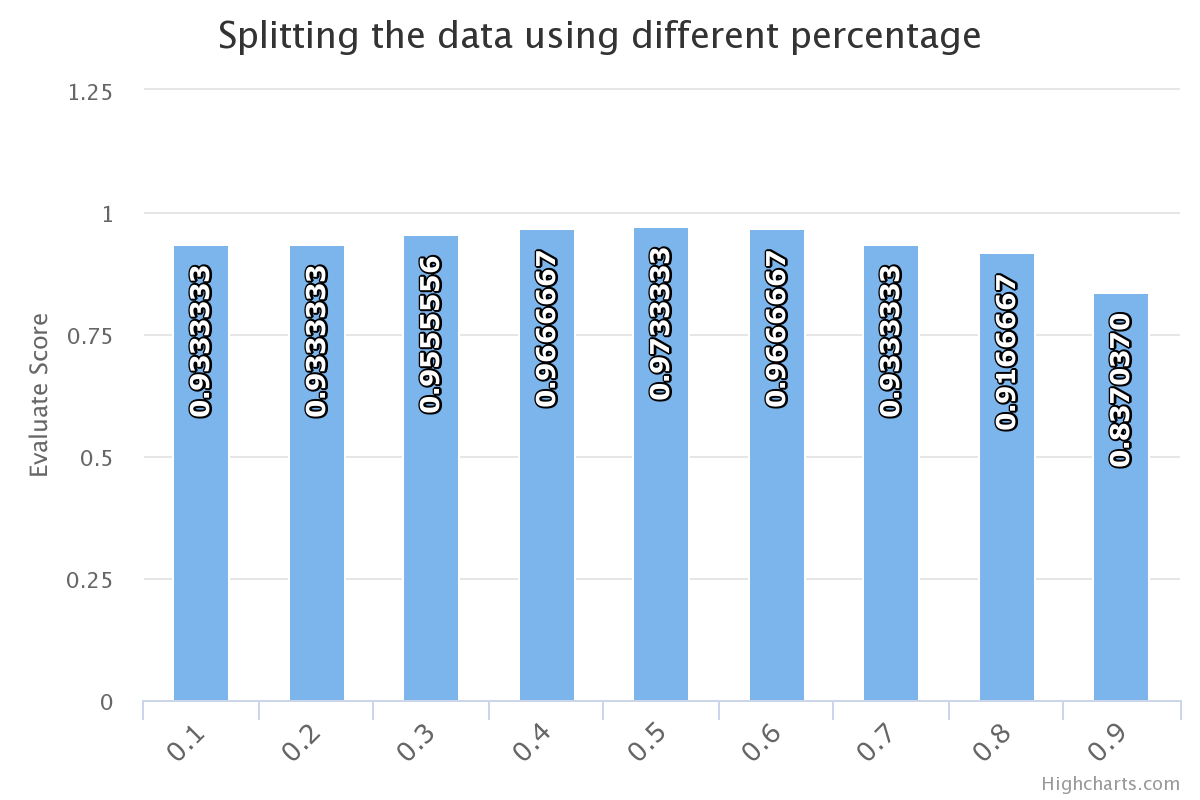
\includegraphics[width=\linewidth]{split.png}
\centerline{fig.1}

\section{Problem two/three}

\begin{table}[h]  
	\centering  
	\caption{cross validation folds}  
	\begin{tabular}{cccc} 
		\hline
		\hline
		& cv's folder & Accuracy  \\ [0.5ex] 
		\hline
		& 2 & 0.94(+/-0.04)   \\
		& 3 & 0.99(+/-0.02)  \\
		& 4 & 0.97(+/-0.04)  \\
		& 5 & 0.97(+/-0.05)  \\
		& 6 & 0.97(+/-0.07) \\
		& 7 & 0.97(+/-0.07) \\
		& 8 & 0.97(+/-0.08) \\

		\hline
		\hline
	\end{tabular}
\end{table}

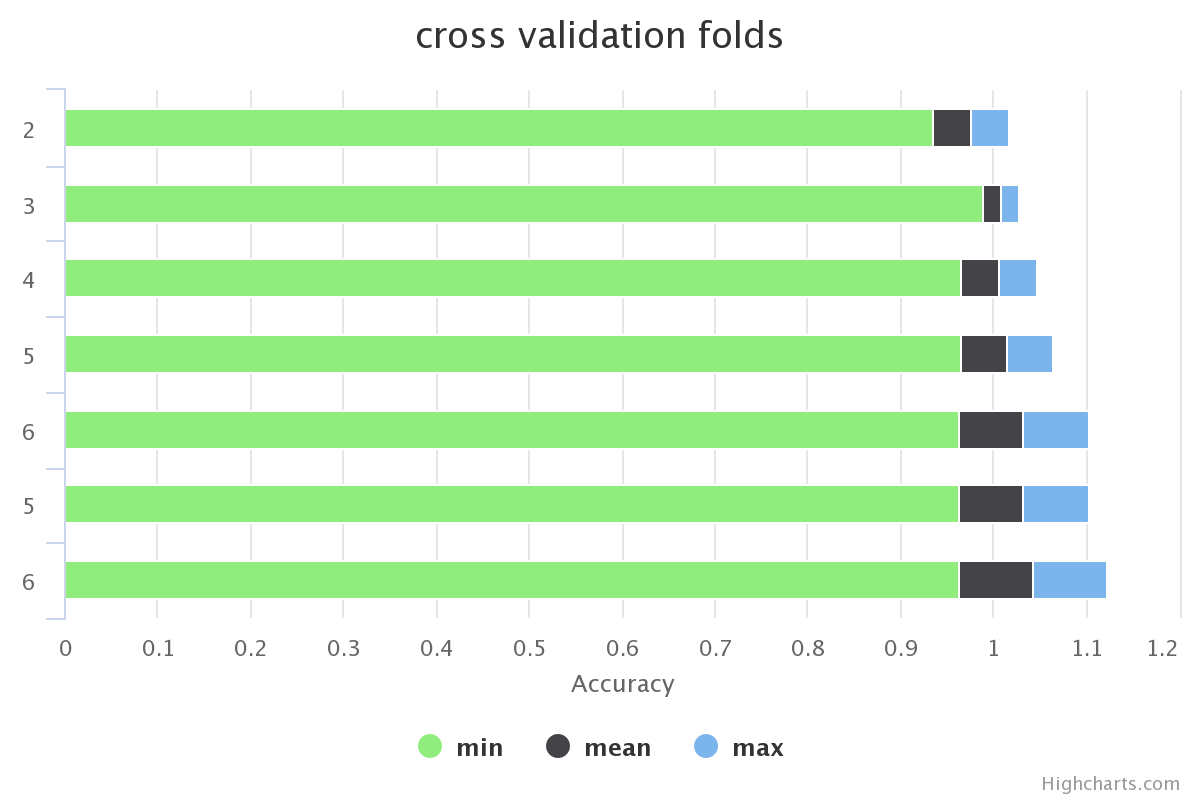
\includegraphics[width=\linewidth]{cross.png}
\centerline{fig.2}

\section{Problem Four}
\begin{table}[h]  
	\centering  
	\caption{Normalise the data}  
	\begin{tabular}{cccc} 
		\hline
		\hline
		& Method & Accuracy  \\ [0.5ex] 
		\hline
		& Min-Max scaling & 0.97(+/-0.05)   \\
		& Standardization & 0.97(+/-0.02)  \\
		& Normalizer & 0.97(+/-0.04)  \\
		\hline
		\hline
	\end{tabular}
\end{table}


\section{Classification}

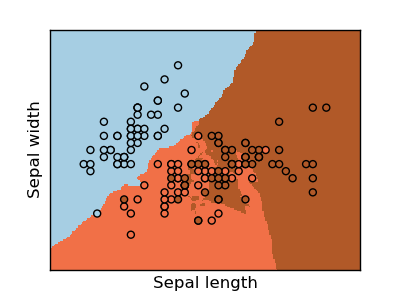
\includegraphics[width=\linewidth]{plot_knn_iris_1.png}
\centerline{fig.2}

split.py\\
To implement Splitting the data using different percentage
\begin{python}
import numpy as np
import pandas as pd
from sklearn import datasets
from sklearn.neighbors import KNeighborsClassifier

iris=datasets.load_iris()
iris_x=iris.data
iris_y=iris.target

# Split iris data in train and test data
# A random permutation, to split the data randomly

np.random.seed(0)
indices=np.random.permutation(len(iris_x))
for i in np.arange(0.1,1,0.1):
test_size=-1*i*len(indices)
test_size=int(test_size)
iris_x_train=iris_x[indices[:test_size]]
iris_y_train=iris_y[indices[:test_size]]
iris_x_test=iris_x[indices[test_size:]]
iris_y_test=iris_y[indices[test_size:]]
#Create a nearest-neighbor classifier
knn=KNeighborsClassifier()
knn.fit(iris_x_train,iris_y_train)
#iris_x_predict=knn.predict(iris_x_test)
#print(iris_x_predict)
#print(iris_y_test)
score=knn.score(iris_x_test,iris_y_test)
#print(score)
print('test proprotion: {0},\nevaluate score:{1}'.format(i,score))
print('-------------------------------------------------')
\end{python}

crossVal.py\\

To use cross validation folds.

\begin{python}
import numpy as np
import pandas as pd
from sklearn import datasets
from sklearn.neighbors import KNeighborsClassifier
from sklearn.model_selection import train_test_split
from sklearn.model_selection import cross_val_score

#Create the KNNClassifer
knn=KNeighborsClassifier()
# knn.fit(x_train,y_train)
for i in range(2,9):
scores=cross_val_score(knn,iris.data,iris.target,cv=i)
print(scores)
print("Accuracy:%0.2f(+/-%0.2f)"%(scores.mean(),scores.std()*2))
print("----------------------------------------------")
\end{python}


normalize.py\\

To normalize the data to train.

\begin{python}
import numpy as np
import pandas as pd
from sklearn import datasets
from sklearn.neighbors import KNeighborsClassifier
from sklearn.model_selection import train_test_split
from sklearn.model_selection import cross_val_score
from sklearn.preprocessing import MinMaxScaler
from sklearn.preprocessing import StandardScaler
from sklearn.preprocessing import Normalizer

iris=datasets.load_iris()
#Min-Max scaling
#MinMaxScaler().fit_transform(iris.data)

#Standardization
# StandardScaler().fit_transform(iris.data)

# Normalizer
Normalizer().fit_transform(iris.data)

# Here we split the data 0.6:0.4
x_train,x_test,y_train,y_test=train_test_split(
iris.data,iris.target,test_size=0.4,random_state=0)

#Create the KNNClassifer
knn=KNeighborsClassifier()
scores=cross_val_score(knn,iris.data,iris.target,cv=5)
print("Accuracy:%0.2f(+/-%0.2f)"%(scores.mean(),scores.std()*2))
\end{python}

plot.py\\

To plot the classification.

\begin{python}
import numpy as np
import pylab as pl
from sklearn import neighbors, datasets

# import some data to play with
iris = datasets.load_iris()
X = iris.data[:, :2] # we only take the first two features. 
Y = iris.target


h = .02 # step size in the mesh

knn=neighbors.KNeighborsClassifier()

# we create an instance of Neighbours Classifier and fit the data.
knn.fit(X, Y)

# Plot the decision boundary. For that, we will asign a color to each
# point in the mesh [x_min, m_max]x[y_min, y_max].
x_min, x_max = X[:,0].min() - .5, X[:,0].max() + .5
y_min, y_max = X[:,1].min() - .5, X[:,1].max() + .5
xx, yy = np.meshgrid(np.arange(x_min, x_max, h), np.arange(y_min, y_max, h))
Z = knn.predict(np.c_[xx.ravel(), yy.ravel()])

# Put the result into a color plot
Z = Z.reshape(xx.shape)
pl.figure(1, figsize=(4, 3))
pl.set_cmap(pl.cm.Paired)
pl.pcolormesh(xx, yy, Z)

# Plot also the training points
pl.scatter(X[:,0], X[:,1],c=Y )
pl.xlabel('Sepal length')
pl.ylabel('Sepal width')

pl.xlim(xx.min(), xx.max())
pl.ylim(yy.min(), yy.max())
pl.xticks(())
pl.yticks(())

pl.show()	
\end{python}
\end{document}